\documentclass{article}
\usepackage{amsmath}
\usepackage{fourier}
\usepackage[pdftex]{graphicx}
\usepackage{epstopdf}
\DeclareGraphicsRule{*}{mps}{*}{} 
%\usepackage{graphicx}
\usepackage{amsmath, amsthm, amssymb}
\usepackage{listings}
\usepackage{float}
\usepackage{enumerate}
\usepackage{hyperref}
\usepackage{fancyheadings}
\usepackage{titlesec}
\usepackage{multicol}
\usepackage{wrapfig}
\usepackage{tocloft}
\usepackage{tikz}
\usepackage{caption}
\usepackage{subcaption}
\usepackage{array}
\usepackage{multirow}

\begin{document}

\chapter{Uncertainty and Error}

\section{Introduction}

There is no such thing as a perfect measurement. All measurements have errors and uncertainties, no matter how hard we might try to minimize them. Understanding possible errors is an important issue in any experimental science. The conclusions we draw from the data, and especially the strength of those conclusions, will depend on how well we control the uncertainties. \myskip

Let’s look at an \emph{example}: You measure two values 2.5 and 1.5. From theory, the expected value is 2.3, so the value 2.5 almost agrees, whereas 1.5 is far off. But if you take into account the uncertainties (i.e.\ the interval in which your result is expected to lie), neither may be far off. For experimental uncertainties of 0.1 and 1.0, respectively, your two measured values may be expressed $2.5\pm 0.1$ and $1.5\pm 1.0$. The expected value falls within the range of the second measurement but not of the first! \myskip

This first lab deals exclusively with this important subject. The techniques studied here will be essential for the rest of this two-semester lab course. The issues are important in order to arrive at good judgments in any field (like medicine) in which it is necessary to understand not just numerical results, but the uncertainties associated with those results.

\section{Theory}

\subsection{Types of Uncertainties}

Uncertainty in a measurement can arise from three possible origins: the measuring device, the procedure of how you measure, and the observed quantity itself. Usually the largest of these will determine the uncertainty in your data. \myskip

Uncertainties can be divided into two different types: systematic uncertainties and random uncertainties. 

\subsubsection{Systematic Uncertainties}

Systematic uncertainties or systematic errors always bias results in one specific direction. They will cause your measurement to consistently be higher or lower than the accepted value. \myskip

An \emph{example} of a systematic error follows. Assume you want to measure the length of a table in cm using a meter stick. However, the stick is made of metal that has contracted due to the temperature in the room, so that it is less than one meter long. Therefore, all the intervals on the stick are smaller than they should be. Your numerical value for the length of the table will then always be larger than its actual length no matter how often or how carefully you measure. Another example might be measuring temperature using a mercury thermometer in which a bubble is present in the mercury column. \myskip

Systematic errors are usually due to imperfections in the equipment, improper or biased observation, or the presence of additional physical effects not taken into account. (An example might be an experiment on forces and acceleration in which there is friction in the setup and it is not taken into account!) \myskip

In performing experiments, try to estimate the effects of as many systematic errors as you can, and then remove or correct for the most important. By being aware of the sources of systematic error beforehand, it is often possible to perform experiments with sufficient care to compensate for weaknesses in the equipment.

\subsubsection{Random Uncertainties}

In contrast to systematic uncertainties, random uncertainties are an unavoidable result of measurement, no matter how well designed and calibrated the tools you are using. Whenever more than one measurement is taken, the values obtained will not be equal but will exhibit a spread around a mean value, which is considered the most reliable measurement. That spread is known as the random uncertainty. Random uncertainties are also unbiased -- meaning it is equally likely that an individual measurement is too high or too low. \myskip

From your everyday experience you might be thinking, ``Stop! Whenever I measure the length of a table with a meter stick I get exactly the same value no matter how often I measure it!''   This may happen if your meter stick is insensitive to random measurements, because you use a coarse scale (like $\mathrm{mm}$) and you always read the length to the nearest $\mathrm{mm}$. But if you would use a meter stick with a finer scale, or if you interpolate to fractions of a millimeter, you would definitely see the spread. As a general rule, if you do not get a spread in values, you can improve your measurements by using a finer scale or by interpolating between the finest scale marks on the ruler. \myskip

How can one reduce the effect of random uncertainties?  Consider the following \emph{example}. Ten people measure the time of a sprinter using stopwatches. It is very unlikely that each of the ten stopwatches will show exactly the same result. Even if all of the people started their watches at exactly the same time (unlikely) some of the people will have stopped the watch early, and others may have done so late. You will observe a spread in the results. If you \emph{average} the times obtained by all ten stop watches, the \emph{mean} value will be a better estimate of the true value than any individual measurement, since the uncertainty we are describing is random, the effects of the people who stop early will compensate for those who stop late. In general, making multiple measurements and averaging can reduce the effect of random uncertainty. \myskip

\emph{Remark}: We usually specify any measurement by including an estimate of the random uncertainty. (Since the random uncertainty is unbiased we note it with a $\pm$ sign). So if we measure a time of 7.6 seconds, but we expect a spread of about 0.2 seconds, we write as a result:
\begin{equation}
    t = (7.6\pm 0.2)\,\mathrm{s}
\end{equation}
indicating that the uncertainty of this measurement is $0.2\,\mathrm{s}$ or about $3\%$. \myskip

\subsection{Numerical Estimates of Uncertainties}

For this laboratory, we will estimate uncertainties with three approximation techniques, which we describe below. You should note which technique you are using in a particular experiment.

\subsubsection{Upper Bound}

Most of our measuring devices in this lab have scales that are coarser than the ability of our eyes to measure.

\begin{figure}[h]
    \begin{center}
        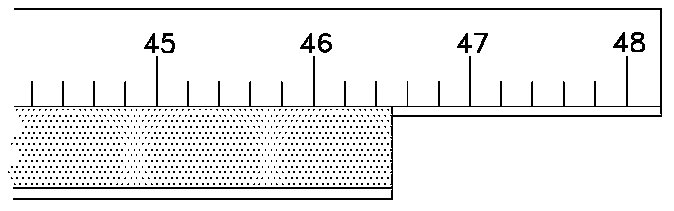
\includegraphics[width=0.5\textwidth]{./Exp1/pic/image1.png}
    \end{center}
    \caption{Measuring Length}
    \label{fig:measure}
\end{figure}

For example in the figure above, where we are measuring the length of an object against a meter stick marked in cm, we can definitely say that our result is somewhere between $46.4\,\mathrm{cm}$ and $46.6\,\mathrm{cm}$. We assume as an \emph{upper} bound of our uncertainty, an amount equal to \emph{half} this width (in this case $0.1\,\mathrm{cm}$). The final result can be written as:
\begin{equation}
    \ell = (46.5\pm 0.1)\,\mathrm{cm}
\end{equation}

\subsubsection{Estimation from the Spread (2/3 method)}

For data in which there is random uncertainty, we usually observe individual measurements to cluster around the mean and drop in frequency as the values get further from the mean (in both directions).\footnote{There is a precise mathematical procedure to obtain uncertainties (standard deviations) from a number of measured values. Here we will apply a simple ``rule of thumb'' that avoids the more complicated mathematics of that technique. The uncertainty using the standard deviation for the group of values in our example below is 0.2.}  Find the interval around the mean that contains about 2/3 of the measured points: \emph{half} the size of this interval is a good estimate of the uncertainty in each measurement. \myskip

The reasons for choosing a range that includes 2/3 of the values come from the underlying statistics of the normal (or Gaussian) distribution. This choice allows us to accurately add and multiply values with errors and has the advantage that the range is not affected much by outliers and occasional mistakes. A range that always includes all of the values is generally less meaningful. \myskip

\emph{Example}: You measure the following values of a specific quantity:
\begin{equation*}
    9.7,\:9.8,\:10,\:10.1,\:10.1,\:10.3
\end{equation*}
The mean of these six values is 10.0. The interval from 9.75 to 10.25 includes 4 of the 6 values; we therefore estimate the uncertainty to be 0.225. The result is that the best estimate of the quantity is 10.0 and the uncertainty of a single measurement is 0.2.\footnote{Note that about 5\% of the measured values will lie \emph{outside} $\pm$ twice the uncertainty}\footnote{While the above method for calculating uncertainty is good enough for our purposes, it oversimplifies a bit the task of calculating the uncertainty of the \emph{mean} of a quantity.  For those who are interested, please see the appendix for elaboration and clarification. }

\subsubsection{Square-Root Estimation in Counting}

For inherently random phenomena that involve counting individual events or occurrences, we measure only a single number $N$. This kind of measurement is relevant to counting the number of radioactive decays in a specific time interval from a sample of material, for example. It is also relevant to counting the number of left-handed people in a random sample of the population. The (absolute) uncertainty of such a single measurement, $N$, is estimated as the square root of $N$. As an example, if we measure 50 radioactive decays in 1 second we should present the result as $50\pm 7$ decays per second. (The quoted uncertainty indicates that a subsequent measurement performed identically could easily result in numbers differing by 7 from 50.)

\subsection{Number of Significant Digits}

The number of significant digits in a result refers to the number of digits that are relevant. The digits may occur after a string of zeroes. For example, the measurement of $2.3\,\mathrm{mm}$ has two significant digits. This does not change if you express the result in meters as $0.0023\,\mathrm{m}$. The number 100.10, by contrast, has 5 significant digits.

When you record a result, you should use the calculated error to determine how many significant digits to keep. Let's illustrate the procedure with the following example. Assume you measure the diameter of a circle to be $d = 1.6232\,\mathrm{cm}$, with an uncertainty of $0.102\,\mathrm{cm}$. You now round your uncertainty to one or two significant digits (up to you). So (using one significant digit) we initially quote $d = (1.6232 \pm 0.1)\,\mathrm{cm}$. Now we compare the mean value with the uncertainty, and keep only those digits that the uncertainty indicates are relevant. Finally, we quote the result as $d = (1.6 \pm 0.1)\,\mathrm{cm}$ for our measurement.

Suppose further that we wish to use this measurement to calculate the circumference $c$ of the circle with the relation $c = \pi\cdot d$. If we use a standard calculator, we might get a 10 digit display indicating:
\begin{equation}
    c = 5.099433195\pm 0.3204424507\,\mathrm{cm}
\end{equation}
This is not a reasonable way to write the result!  The uncertainty in the diameter had only one significant digit, so the uncertainty of the circumference calculated from the diameter cannot be substantially better. Therefore we should record the final result as: 
\begin{equation}
    c = 5.1\pm 0.3\,\mathrm{cm}
\end{equation}
(If you do intermediate calculations, it is a good idea to keep as many figures as your calculator can store. The above argument applies when you \underline{record} your results!)

\subsection{Relative and Absolute Uncertainty}

There are two ways to record uncertainties: the absolute value of the uncertainty or the uncertainty relative to the mean value. So in the example above, you can write $c = (5.1 \pm 0.3)\,\mathrm{cm}$ or equally well $c = 5.1\,\mathrm{cm}\; (1.00 \pm 0.06)$. You can see that if you multiply out the second form you will obtain the first, since $5.1 \times 0.06 = 0.3$. The second form may look a bit odd, but it tells you immediately that the uncertainty is 6\% of the measured value. The number $0.3\,\mathrm{cm}$ is the absolute uncertainty and has the same units as the mean value (cm). The 0.06 (or 6\%) is the relative uncertainty and has no units since it is the ratio of two lengths.

\subsection{Propagation of Uncertainties}

Often, we are not directly interested in a measured value, but we want to use it in a formula to calculate another quantity. In many cases, we measure many of the quantities in the formula and each has an associated uncertainty. We deal here with how to propagate uncertainties to obtain a well-defined uncertainty on a computed quantity. 

\subsubsection{Adding/Subtracting Quantities}

When we \underline{add or subtract} quantities, their uncertainties must always be \underline{added} (never subtracted) to obtain the \underline{absolute uncertainty} on the computed quantity.\footnote{The propagation of random uncertainties is actually slightly more complicated, but the procedure outlined here usually represents a good approximation, and it never underestimates the uncertainty. See the appendix for more information.}

Take as an example measuring the length of a dog. We measure the distance between the left wall and the tail of the dog and subtract the distance from the wall to the dog's nose.
\begin{figure}[h]
    \begin{center}
        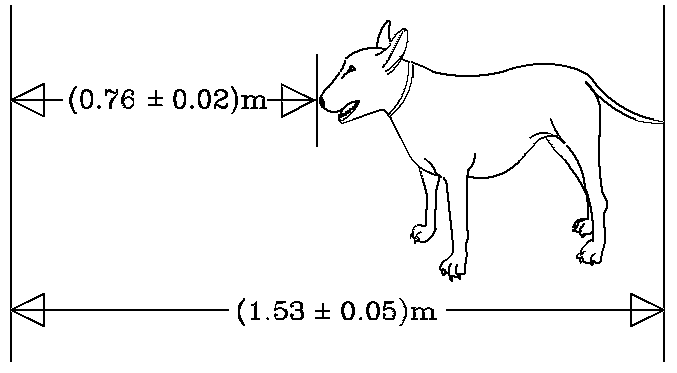
\includegraphics[width=0.5\textwidth]{./Exp1/pic/image2.png}
    \end{center}
    \caption{Measuring a Dog}
    \label{fig:dog}
\end{figure}
So the total length of the dog is:
\begin{equation}
    \begin{split}
        \text{Length} &= (1.53\pm 0.05)\,\mathrm{m} - (0.76 \pm 0.02)\,\mathrm{m} \\
        &= \left( 1.53 - 0.76 \right)\pm\left( 0.05 + 0.02 \right)\,\mathrm{m} \\
        &= \left( 0.77 \pm 0.07 \right)\,\mathrm{m}
    \end{split}
\end{equation}

\subsubsection{Multiplying/Dividing Quantities}

When we \underline{multiply or divide} quantities, we \underline{add} (never subtract) the \underline{relative uncertainties} to obtain the \underline{relative uncertainty} of the computed quantity.\footnote{Our calculation of the uncertainty actually overestimates it. The correct method does not add the absolute/relative uncertainty, but rather involves evaluating the square root of the sum of the squares. For more information please refer to the appendix of this experiment.}

Take as an example the area of a rectangle, whose individual sides are measured to be: 
\begin{align}
    a = 25.0\pm 0.5\,\mathrm{cm} = 25.0\,\mathrm{cm}\;(1.00\pm 0.02) \nonumber \\
    b = 10.0\pm 0.3\,\mathrm{cm} = 10.0\,\mathrm{cm}\;(1.00\pm 0.03)
\end{align}

The area is obtained as follows:
\begin{equation}
    \begin{split}
        \text{Area} &= \left( 25.0\pm 0.5\,\mathrm{cm} \right)\cdot\left( 10.0\pm 0.3\,\mathrm{cm} \right) \\
        &= 25.0\,\mathrm{cm}\;\left( 1.00\pm 0.02 \right)\cdot 10.0\,\mathrm{cm}\;\left( 1.00\pm 0.03 \right) \\
        &= \left( 25.0\,\mathrm{cm}\cdot 10.0\,\mathrm{cm} \right)\left( 1.00\pm \left( 0.02 + 0.03 \right) \right) \\
        &= 250.0\,\mathrm{cm}^2\;(1.00 \pm 0.05) \\
        &= 250.0\pm 12.5\,\mathrm{cm}^2 \\
        &= 250 \pm 10\,\mathrm{cm}^2
    \end{split}
\end{equation}

Note that the final step has rounded both the result and the uncertainty to an appropriate number of significant digits, given the uncertainty on the lengths of the sides. \myskip

\underline{Remarks:} Note that uncertainties on quantities used in a mathematical relationship always increase the uncertainty on the result. The quantity with the biggest uncertainty usually dominates the final result. Often one quantity will have a much bigger uncertainty than all the others. In such cases, we can simply use this main contribution. \myskip



\subsubsection{Powers and Roots}

When raising a value to a certain power, its relative uncertainty is multiplied by the exponent. This applies to roots as well, since taking the root of a number is equivalent to raising that number to a fractional power.\myskip 

Squaring a quantity involves multiplying its relative uncertainty by 2, while cubing a quantity causes its relative uncertainty to be multiplied by 3.\myskip

Taking the \underline{square root} of a quantity (which is equivalent to raising the quantity to the 1/2 power) causes its \underline{relative uncertainty} to be multiplied by 1/2. For example, if you know the area of a square to be: 
\begin{equation}
    \text{Area} = 100\pm 8\,\mathrm{m^2} = 100\,\mathrm{m}^2\;(1.00\pm 0.08)
\end{equation}
then it follows that the side of the square is:
\begin{equation}
    \text{Side} = 10\,\mathrm{m}\;\left( 1.00\pm 0.04 \right) = 10.0\pm 0.4\,\mathrm{m}
\end{equation}
You can convince yourself that this is true by checking it backwards using the rules described in section 2.5.2.

\subsubsection{Multiplication by a Constant}

Multiplying a value by a constant does not change its relative error.

\subsubsection{Other Functions}

If you need to calculate the error of a calculation that does not fit into one of these rules (such as trigonometric functions or logarithmic ones), here is a manual method that you can use.\myskip

Based upon the error of the quantity that you determined, you can find the maximum and minimum values of the quantity that you are calculating. The value that you found should be roughly midway between these two quantities. Then if you split the difference between the maximum and minimum you should obtain a reasonable estimate of the error.\myskip

Here is an example: Suppose you measure an angle to be $(47.3 \pm 0.5)^\circ$ and you want to determine the error of $\sin(47.3 \pm 0.5)^\circ$. You find that $\sin(47.3) = 0.735$. Based upon your reported uncertainty, you know that your angle could be as large as $47.8^\circ$ and as small as $46.8^\circ$, and therefore you should calculate $\sin(47.8) = 0.741$ and $\sin(46.8) = 0.729$. So your calculated value is 0.735 but it can be as low as 0.729 and as high as 0.741 and therefore, if you halve the difference between 0.729 and 0.741 you get a reasonable error estimate of 0.006. So you should report your value as $0.735 \pm 0.006$.

\section{Description and Procedure}

You are to perform two experiments to practice the estimation of uncertainty and the propagation of errors. These involve measuring the period of a pendulum and measuring the reaction time of a human being.

\subsection{Pendulum}

In the first part, we measure the time it takes a pendulum to swing through a full cycle, the period of oscillation, and compare this to the theoretical prediction. Two methods of recording the time will be used to illustrate that different ways of making a measurement can result in very different uncertainties. In each case, many measurements will be taken to demonstrate the frequency of differing values. Since a number of measurements need to be made, you may wish to perform this experiment in teams of two: one person measures the time values, the other records the results. \myskip

In the first series, the stopwatch should be started when the pendulum is at one of its maximum positions and stopped as it returns to that position. A full period should be measured, not the time it takes for the pendulum to travel from one maximum point to the other. After 24 measurements, sort the measurements in bins of $50\,\mathrm{ms}$. (Therefore all measurements with times between e.g.\ $1.25\,\mathrm{s}$ and $1.29\,\mathrm{s}$ (inclusive) are placed in the same bin.)  Make a graph of the frequency of measurements in the bins vs.\ the times of the bins. Calculate the average and estimate the uncertainty using the 2/3 rule.\myskip

In the second series, measure the time as the pendulum passes a fixed characteristic mark in the background. For this you might use a chair or the leg of a table, or the lowest point of the pendulum swing. In order to make sure you are again measuring a complete period, you should take care to measure the time between when the pendulum passes through the same point in the same direction. Perform the same experiment, making 24 measurements, and sort the measurements in bins of $50\,\mathrm{ms}$. Again graph your result and get the average and the uncertainty using the 2/3 estimate.\myskip

See if there is a substantial difference between the uncertainties of these two measurements and also if the measured values (i.e. the averages) coincide within uncertainty. In addition, measure the length $\ell$ of the pendulum from the pivot point to the center of the mass (note that you will need to guess somewhat on the location of the center of the mass). This allows you to determine the acceleration due to gravity at the earth's surface, $g$, using the formula\footnote{This will be covered in the 1201 lecture course. See, for example, Chapter 15 in \emph{Fundamentals of Physics} by Halliday, Resnick \& Walker.}:
\begin{equation}
    \frac{2\cdot \pi}{t} = \sqrt{\frac{g}{\ell}}
\end{equation}
where $t$ is the measured period. Make sure to propagate uncertainty from $\ell$ and $t$. Finally, compare your value of $g$ to the accepted value:
\begin{equation}
    g = 9.8\,\mathrm{m/s^2}
\end{equation}

\begin{itemize}
    \item Does the accepted value of $g$ fall within your uncertainty?
    \item What are the sources of error?
\end{itemize}

\subsection{Reaction Time}

Next measure your reaction time to a specific stimulus. Perform this experiment with a partner, but every student should obtain his/her own data.\myskip

One student holds a meter ruler (vertically) at the upper end and the other student places two fingers around (but not touching) the $50\,\mathrm{cm}$ mark of the ruler. The first student (quietly) releases the ruler and the second student tries to grab it as soon as possible after he/she sees it released. Measure the distance s the ruler falls. After performing this experiment 10 times (for each student), look at the spread in the data and calculate the resulting uncertainty (using the 2/3 estimate). If you have a few values that are far off from all the other values (e.g.\ because you were irritated or distracted) you may decide to ignore them when you calculate your reaction time, but note in your lab report which measured points were not used.\myskip

Use the relation\footnote{See, for example, Chapter 2 in the Halliday, Resnick \& Walker text.}:
\begin{equation}
    s = \frac{1}{2}g\cdot t^2
\end{equation}
to calculate your average reaction time and the corresponding uncertainty. This experiment is an example of an indirect measurement. You measure a quantity (here the distance the ruler is falling) that you do not care about directly, but is necessary in order to calculate the quantity you want to know (the reaction time).\myskip

You should report your reaction time in seconds in your lab report.

\begin{itemize}
    \item Would it be reasonable to give your measured values with a precision measured in millimeters? Why or why not?
    \item How well could you get the same initial conditions for each try?
    \item Note the major sources of error.
    \item Suggest improvements to the lab or shortly describe a better experiment.
\end{itemize}
\newpage
\section{Sample Data Sheet}

\subsection{Pendulum}

Length of the pendulum $\qquad = $ \hspace{2cm} $\pm$ \hspace{2cm} $\mathrm{cm}$

\begin{multicols}{2}
    From Max to Max

    \vspace{0.5cm}
    \begin{tabular}{|c|}
        \hline \hspace{2cm} \\ \hline \hspace{2cm} \\ \hline \hspace{2cm} \\ \hline \hspace{2cm} \\ \hline \hspace{2cm} \\ \hline \hspace{2cm} \\ \hline \hspace{2cm} \\ \hline \hspace{2cm} \\ \hline \hspace{2cm} \\ \hline \hspace{2cm} \\ \hline \hspace{2cm} \\ \hline \hspace{2cm} \\ \hline \hspace{2cm} \\ \hline \hspace{2cm} \\ \hline \hspace{2cm} \\ \hline \hspace{2cm} \\ \hline \hspace{2cm} \\ \hline \hspace{2cm} \\ \hline \hspace{2cm} \\ \hline \hspace{2cm} \\ \hline \hspace{2cm} \\ \hline \hspace{2cm} \\ \hline \hspace{2cm} \\ \hline \hspace{2cm} \\ \hline \hspace{2cm} \\ \hline
    \end{tabular}

    Using Reference Point

    \vspace{0.5cm}
    \begin{tabular}{|c|}
        \hline \hspace{2cm} \\ \hline \hspace{2cm} \\ \hline \hspace{2cm} \\ \hline \hspace{2cm} \\ \hline \hspace{2cm} \\ \hline \hspace{2cm} \\ \hline \hspace{2cm} \\ \hline \hspace{2cm} \\ \hline \hspace{2cm} \\ \hline \hspace{2cm} \\ \hline \hspace{2cm} \\ \hline \hspace{2cm} \\ \hline \hspace{2cm} \\ \hline \hspace{2cm} \\ \hline \hspace{2cm} \\ \hline \hspace{2cm} \\ \hline \hspace{2cm} \\ \hline \hspace{2cm} \\ \hline \hspace{2cm} \\ \hline \hspace{2cm} \\ \hline \hspace{2cm} \\ \hline \hspace{2cm} \\ \hline \hspace{2cm} \\ \hline \hspace{2cm} \\ \hline \hspace{2cm} \\ \hline
    \end{tabular}
\end{multicols}

\subsection{Reaction Time}

\begin{tabular}[h]{|c|c|c|c|c|c|c|c|c|c|}
    \hline
    1\ & \hspace{1.5cm} &2\ & \hspace{1.5cm} &3\ & \hspace{1.5cm} &4\ & \hspace{1.5cm} &5\ & \hspace{1.5cm} \\ \hline
    6\ & \hspace{1.5cm} &7\ & \hspace{1.5cm} &8\ & \hspace{1.5cm} &9\ & \hspace{1.5cm} &10\ & \hspace{1.5cm} \\ \hline
\end{tabular}

\section{Applications}

You read of a certain test intended to indicate a particular kind of cancer. The test gives you a positive result for $(80 \pm 10) \%$ of all persons tested who really have this kind of cancer (true positives). But the test also gives you a positive result for $(2 \pm 1) \%$ of all healthy persons (false positives). Now you read a publication where the author performed this test on $10,000$ workers that deal with a certain chemical. The author got 400 positive samples from these workers and claims that this is strong evidence that this particular chemical enhances the development of this kind of cancer since it is known from literature that only $(1 \pm 0.5)\%$ of the population are expected to have this kind of cancer. How reliable is the claim of the author?\myskip

\noindent \underline{Numerical Answer}:

If one assumes that the 10,000 workers would mirror the average population, then there should be:
\begin{equation}
    10000\pm(0.010 \pm 0.005) = 100 \pm 50
\end{equation}
persons having this cancer. Of them, the test gives:
\begin{equation}
    (0.8 \pm 0.1)\pm(100 \pm 50) = 80 \pm 50
\end{equation}
positive results (true positives).\myskip

There are then $9900 \pm 50$ persons expected not to have this kind of cancer. Of them:
\begin{equation}
    (0.02 \pm 0.01)\pm(9900 \pm 50) \approx 200 \pm 100
\end{equation}
give positive results (false positives).\myskip

The total number of positives in the average population is therefore $280 \pm 150$.\myskip

So how do you judge the author's conclusion of ``strong evidences''?\myskip

If you wanted to design a new test using the same procedure but to arrive at a stronger conclusion, and you could either increase the rate of true positives or decrease the rate of wrong negatives, which would you choose?\myskip

\noindent\emph{Reference}: Paul Cutler: Problem Solving in Clinical Medicine, Chapter 5, Problem 5 (modified).

\section{Lab Preparation Examples}

Below are some questions to help you prepare. You will \underline{not} be expected to answer all these questions as part of your lab report. \myskip

\noindent \underline{Estimation of Uncertainty}:\myskip

1. You have the following distribution of measured values:
\begin{table}[h]
    \centering
    \begin{tabular}{|c|l|l|l|}
        \hline
         %& 5 & 10 & 15 \\ \hline
        \quad 0\quad & \hspace{1.5cm} & \hspace{1.5cm} & \hspace{1.5cm} \\ \hline
        \quad 1\quad & I & \hspace{1.5cm} & \hspace{1.5cm} \\ \hline
        \quad 2\quad & III & \hspace{1.5cm} & \hspace{1.5cm} \\ \hline
        \quad 3\quad & IIIII & I & \hspace{1.5cm} \\ \hline
        \quad 4\quad & IIIII & IIII & \hspace{1.5cm} \\ \hline
        \quad 5\quad & IIIII & IIIII & IIIII \\ \hline
        \quad 6\quad & IIIII & IIIII & I \\ \hline
        \quad 7\quad & IIIII & III & \hspace{1.5cm} \\ \hline
        \quad 8\quad & IIII & \hspace{1.5cm} & \hspace{1.5cm} \\ \hline
        \quad 9\quad & II & \hspace{1.5cm} & \hspace{1.5cm} \\ \hline
        \quad 10\quad & I & \hspace{1.5cm} & \hspace{1.5cm} \\ \hline
    \end{tabular}
\end{table}

Estimate the uncertainty using the 2/3 estimate. \myskip

2. Estimate the mean and uncertainty of the following group of values:
\begin{equation*}
    1.6\,\mathrm{s}, 1.3\,\mathrm{s}, 1.7\,\mathrm{s}, 1.4\,\mathrm{s}
\end{equation*}

3. In a radioactive decay you get 16 counts. What is the absolute uncertainty of the number of counts? What is the relative uncertainty? \myskip

4. In a radioactive decay you get 1600 counts. What is the absolute uncertainty of the number of counts? What is the relative uncertainty? \myskip

5. How many counts should you get so that the relative uncertainty is $1\%$ or less? \myskip

\noindent \underline{Significant digits}: \myskip

6. How many significant digits has $l = 0.0254\,\mathrm{m}$? \myskip

7. Write $t = 1.25578 \pm 0.1247\,\mathrm{s}$ with two significant digits (in the uncertainty). \myskip

\noindent \underline{Propagation of Uncertainty}: \myskip

8. For a pendulum with $l = 1.0 \pm 0.1\,\mathrm{m}$, you measure a period of $t = 2.0 \pm 0.2\,\mathrm{s}$. What is the value of the earth's acceleration g? \myskip

9. You measure the volume of a box by measuring the length of the single sides. For the lengths of the single sides you get:
\begin{equation*}
    a = 10.0 \pm 0.1\,\mathrm{cm}\qquad    b = 5.0 \pm 0.2\,\mathrm{cm} \qquad c = 7.5 \pm 0.3\,\mathrm{cm}
\end{equation*}
What is the volume of the box (including uncertainty and units) in $\mathrm{cm}^3$? What is the volume of the box in $\mathrm{m}^3$? \myskip

10. You measure the following quantities:
\begin{align*}
    A &= 1.0 \pm 0.2\,\mathrm{m}\quad B = 2.0 \pm 0.2\,\mathrm{m}\quad        C = 2.5 \pm 0.5\,\mathrm{m/s} \\ 
    D &= 0.10\pm 0.01\,\mathrm{s}\quad E = 100\pm 10\,\mathrm{m/s^2} &
\end{align*}
Calculate the mean and uncertainty of:
\begin{enumerate}[a)]
    \item $A+B=$
    \item $A-B=$
    \item $C\cdot D=$
    \item $C/D=$
    \item $C\cdot D + A=$
    \item $\frac{1}{2}E\cdot D + C=$
    \item $A\cdot B/(A-B)=$
\end{enumerate}
Include units! For e)--g) perform it step by step.\myskip

\noindent \underline{Relative and Absolute Uncertainty}:\myskip

11. What is the relative uncertainty for $v = 12.25 \pm 0.25\,\mathrm{m/s}$?\myskip

12. What is the absolute uncertainty if the mean value is $120\,\mathrm{s}$ and the relative uncertainty is $5\%$?\myskip

13. Given the following measurements, which one has the highest absolute uncertainty and which one has the highest relative uncertainty?
\begin{align*}
    l &= 10.0 \pm 0.2\,\mathrm{m} \quad   l = 10.0\,\mathrm{m}\: (1.00 \pm 0.03)   \\ 
    l &= 7.24\,\mathrm{m}\: (1.00 \pm 0.04) \quad l = 12.5 \pm 0.25\,\mathrm{m}   
\end{align*}

14. Given the following measurements which one has the highest absolute uncertainty and which one has the highest relative uncertainty?\myskip
\begin{align*}
    l &= 10.0\pm 0.2\,\mathrm{m} \quad t = 7.5\pm 0.2\,\mathrm{s} \\
    d &= 5.6\,\mathrm{cm}\:(1.00\pm 0.04) \quad v = 6.4\times 10^6\,\mathrm{m/s}\:(1.00\pm 0.03)
\end{align*}
\emph{Caution}: Don't get tricked!\myskip

\noindent \underline{Explanations}:\myskip

15. Explain, using your own words, why the uncertainty decreases as you average over several measurements (you might want to take a look at the appendix).\myskip

%16. Explain, using your own words, the difference between uncertainty and error as you perform several measurements and average.\myskip

16. You measure the speed of light and get as a result $c = (2.25 \pm 0.25)\times 108\,\mathrm{m/s}$. The value you find in books is $c = 299\, 792\, 458\,\mathrm{m/s}$.  Using these values explain the difference between the uncertainty of your measurement and its error!

\section{Appendix}
\subsection{Clarification of 2/3 Rule}

To find the true uncertainty, we are really interested in the \emph{standard error of the mean}, i.e. how likely it would be for a newly measured average value to be close to our original value were we to perform the experiment again.  The proper way to figure this out would be to get say a thousand friends to perform this experiment in the same way, each using the same number of data points, and then compare the results of everyone.  Each student would calculate his or her own mean, and they would likely all be clustered around some central average.  We could then examine the spread of this cluster of means using the 2/3 rule, and we'd have a quantitative measure of the uncertainty surrounding any single student's measurement.\myskip

While it's usually impractical to get 1000 friends together to repeat an experiment a thousand times, it turns out that the uncertainty (or ``standard error'') of the mean can be estimated with the following formula:
\begin{equation}
    \text{Standard Error Of The Mean} = \frac{\text{Uncertainty Of Single Measurement}}{\sqrt{N}}
\end{equation}
where ``$N$'' is the number of data points in your sample, and ``Uncertainty Of Single Measurement'' is the uncertainty calculated via the 2/3 method.  The ``$\sqrt{N}$'' term should make sense qualitatively -- as we take more and more data points, our measured average becomes less and less uncertain as we approach what should be the ``global'' mean.

\subsection{The ``Correct'' Way to Add Uncertainties}

The rules we've given for propagating uncertainties through a calculation are essentially correct, and intuitively make sense.  When adding two quantities together, if one has an uncertainty of $\Delta$x and another has an uncertainty of $\Delta y$, the sum could indeed range from $(x+y) - (\Delta x +  \Delta y)$ to $(x+y) + (\Delta x + \Delta y)$.  This implies that the proper way to find the uncertainty of $(x+y)$ is to add their respective absolute uncertainties. \myskip

There is, however, a small problem -- this overestimates the uncertainty!  Since $x$ and $y$ are equally likely to be wrong by either a \emph{positive} amount or a \emph{negative} amount, there's a good chance that the respective errors of each variable will partly cancel one another out.  To account for this, a more accurate way to estimate uncertainty turns out to be to add uncertainties \emph{in quadrature}.  This means:\myskip

\textbf{Adding/Subtracting Quantities}

\begin{equation}
    (A\pm\Delta A) + (B\pm\Delta B) = (A+B)\pm\sqrt{(\Delta A)^2+(\Delta B)^2}
\end{equation}

\myskip\textbf{Multiplying/Dividing Quantities}
\phantom{AAAA AAA AAAA AA AAA AAAA AAAA AAAAAAA AAA AAAA AAAA AAAA AAAAA AAAAA AAAAA AAAAAA AAAAAAA AAAAA AAA AAA AAAAA AAAAA AAAAA AAAAA AAAAA AAAAA AAAAA AAAAA AAAAA AAAAA AAAAA AAAAA AAAAA AAAAA AAAAAA}

\begin{equation}
    A\left(1\pm\frac{\Delta A}{A}\right) \times B\left(1\pm\frac{\Delta B}{B}\right) = \left(A \times B\right) \left ( 1 \pm\sqrt{\left(\frac{\Delta A}{A}\right)^2+\left(\frac{\Delta B}{B}\right)^2} \right )
\end{equation}

While this method gives a closer approximation to what the true propagated uncertainty should be, it is clearly a more complex calculation.  In the limited time available to complete your experiment and lab report, you may use the simpler, earlier uncertainty calculation method provided, and avoid this complicated calculation.  But do remember that the simpler method \emph{overestimates} the total uncertainty.


\section{Comments for TA}
\subsection{Required Error Propagation}
\begin{enumerate}
\item Calculate error in the gravitational constant $g$ by propagating uncertainties in period $\tau$ and length $l$. Do this for both $\tau$ measurements.
\item Calculate error in reaction time by propagating uncertainties in distance $s$. Find the uncertainty in distance using the 2/3 estimate.
\end{enumerate}

\subsection{Required Prelab Questions}
\begin{enumerate}
\item Complete prelab questions 5, 8, 9, 13, 15.
\end{enumerate}

\subsection{Additional Comments}
\begin{enumerate}
\item Suggest that students allow the pendulum to oscillate for 5 full periods before measurement to ensure simple harmonic motion.
\end{enumerate}

\end{document}
